% !TeX spellcheck = en_B
% !TeX encoding = UTF-8
\documentclass[8pt]{beamer}

\usepackage[utf8]{inputenc}                                                     
 \usetheme[block=fill,progressbar=foot,background=light]{metropolis}                                                               
%  \usecolortheme{crane}                                                       
  %\useinnertheme{circles}                                                         
  \usepackage[english]{babel}                                                     
  \usepackage{csquotes}                                                           
  \usepackage[T1]{fontenc}                                                        
  \usepackage{booktabs}                                                       \usepackage{pgfgantt}
  \usepackage{pifont}
  \usepackage{adfbullets}
  \usepackage{enumitem}
  \usepackage{amsmath}   
  \usepackage{tikz}
  \usepackage{amssymb}
  \usepackage{amsfonts}
  \usepackage{mathrsfs}   
  \usepackage{graphicx}
  \usepackage{adjustbox}
  \usepackage{varioref}
  \usepackage{probsoln}
  \usepackage{attachfile2}
  \usepackage{pgfplots}
\pgfplotsset{compat=newest}
  \usepackage[style=authoryear,backref=true]{biblatex}
 \usepackage[]{hyperref} 
  \graphicspath{{Graphics/}}
  \usepackage{multirow,array}
  \addbibresource{../Everything.bib}
  \usepackage{colortbl}
  \definecolor{aa}{RGB}{255, 124, 0}
  \definecolor{cc}{RGB}{230, 230, 230}    
  %\setbeamercolor{palette tertiary}{fg=aa,bg=cc}
  %\setbeamercolor{structure}{fg=cc}
  %\setbeamercolor{alerted text}{fg=red}
  
  %Information to be included in the title page:
  
  \usebackgroundtemplate{%
  \tikz[overlay,remember picture]{\node[scale=80,opacity=0.03, at=(current page.south east)] {\adfbullet{9}};}}
  
  \author[]{T. Bretschneider}
  
  \date[\today]{\today}

\usepackage{comment}
\usepackage{varwidth}

\newcommand{\mat}[4]{\left(\begin{array}{cc} #1 & #2 \\ #3 & #4 \\ \end{array}\right)}
\newcommand{\Q}{\mathbb{Q}}
\newcommand{\R}{\mathbb{R}}
\newcommand{\Z}{\mathbb{Z}}
\newcommand{\sol}[2][+]{
	\tikz[baseline]{\node[color=aa,fill=cc,rectangle,draw,anchor=base] {  {\onslide<#1->{#2}}  };}
}

\usetikzlibrary{positioning}
\usetikzlibrary{tikzmark}
\usetikzlibrary{shadings}
\usetikzlibrary{through}


\def\height{0.8cm}
\def\width{1.2cm}

		\newcommand{\keynode}[6]{\node[minimum height=\height,minimum width=\width,draw,rectangle,color=aa,fill=cc] (#3) at (#1,#2) {};
	\node[rectangle,minimum height=\height/2,minimum width=\width,above,color=aa] at (#3) {#3};
	\node[draw,rectangle,minimum height=\height/2,minimum width=\width/3,below,color=aa,fill=cc,inner sep =0cm] at (#3) {\footnotesize#4};
	\node[draw,rectangle,minimum height=\height/2,minimum width=\width/3,below,xshift=\height/2,color=aa,fill=cc,inner sep=0cm] at (#3) {\footnotesize#5};
	\node[draw,rectangle,minimum height=\height/2,minimum width=\width/3,below,xshift=-\height/2,color=aa,fill=cc,inner sep=0cm] at (#3) {\footnotesize#6}; }

\newenvironment{gantt}[3]{\begin{ganttchart}[#1,bar height=.6,bar top shift=.2,title/.style=  {draw=none},y unit chart=0.6cm,y unit title = 0.6cm,include title in canvas=false,group/.append style={draw=black,dashed},bar/.append style={fill=aa},inline,hgrid=true,Float1/.style={bar/.append style={fill=none,dashed},bar height=.8,bar top shift=0.1}]{#2}{#3}}{\end{ganttchart}}

\newenvironment{nicetable}[1]{\setlength\arrayrulewidth{0.5mm}
			\arrayrulecolor{white}
			\begin{tabular}{#1}}{\end{tabular}}
		
\setlist[itemize,1]{label={\color{aa}\huge\adfbullet{9}}}
\setlist[itemize, 2]{label={\color{aa}\large\adfbullet{9}}}

\newcommand\reshist{}
\def\reshist(#1)#2(#3)#4(#5)%
{\draw (axis cs:#1) rectangle (axis cs:#3) node [midway] {#5};}






\title[Discrete]{{\color{aa}\Huge\adfbullet{9}}AL FM Discrete}
\subtitle{Graph Isomorphism and Planar Graphs, \textattachfile{GraphIsomorphismandPlanarGraphs.tex}{(TeX)}}

\begin{document}
	
\setlength{\abovedisplayskip}{0pt}
\setlength{\belowdisplayskip}{0pt}
\setlength{\abovedisplayshortskip}{0pt}
\setlength{\belowdisplayshortskip}{0pt}

\frame{\titlepage}

\begin{frame}{Graph Isomorphism}
	\begin{alertblock}{Isomorphic}
	Two graphs are said to be \textbf{isomorphic} if they have the same number of vertices connected in the same way. 
\end{alertblock}

The following graphs would all be isomorphic.
\begin{center}
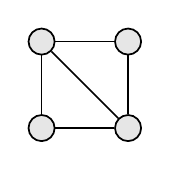
\begin{tikzpicture}[scale=0.5]
[every node/.style={inner sep=0pt}]
\node (1) [circle, minimum size=6pt, fill=cc, line width=0.625pt, draw=black] at (112.5pt, -125.0pt)  {};
\node (2) [circle, minimum size=6pt, fill=cc, line width=0.625pt, draw=black] at (175.0pt, -125.0pt)  {};
\node (3) [circle, minimum size=6pt, fill=cc, line width=0.625pt, draw=black] at (175.0pt, -187.5pt)  {};
\node (4) [circle, minimum size=6pt, fill=cc, line width=0.625pt, draw=black] at (112.5pt, -187.5pt)  {};
\draw [line width=0.625, color=black] (1) to  (3);
\draw [line width=0.625, color=black] (2) to  (3);
\draw [line width=0.625, color=black] (2) to  (1);
\draw [line width=0.625, color=black] (1) to  (4);
\draw [line width=0.625, color=black] (4) to  (3);
\end{tikzpicture}
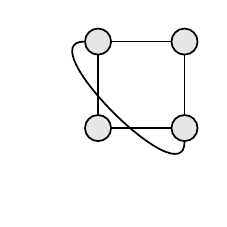
\begin{tikzpicture}[scale=0.5]
[every node/.style={inner sep=0pt}]
\node (1) [circle, minimum size=6pt, fill=cc, line width=0.625pt, draw=black] at (112.5pt, -125.0pt)  {};
\node (2) [circle, minimum size=6pt, fill=cc, line width=0.625pt, draw=black] at (175.0pt, -125.0pt)  {};
\node (3) [circle, minimum size=6pt, fill=cc, line width=0.625pt, draw=black] at (175.0pt, -187.5pt)  {};
\node (4) [circle, minimum size=6pt, fill=cc, line width=0.625pt, draw=black] at (112.5pt, -187.5pt)  {};
\draw [line width=0.625, color=black] (1) to  [in=270, out=180] (3);
\draw [line width=0.625, color=black] (2) to  (3);
\draw [line width=0.625, color=black] (2) to  (1);
\draw [line width=0.625, color=black] (1) to  (4);
\draw [line width=0.625, color=black] (4) to  (3);
\end{tikzpicture}
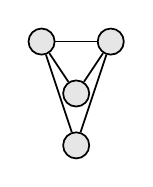
\begin{tikzpicture}[scale=0.5]
[every node/.style={inner sep=0pt}]
\node (1) [circle, minimum size=6pt, fill=cc, line width=0.625pt, draw=black] at (112.5pt, -125.0pt)  {};
\node (3) [circle, minimum size=6pt, fill=cc, line width=0.625pt, draw=black] at (162.5pt, -125.0pt)  {};
\node (2) [circle, minimum size=6pt, fill=cc, line width=0.625pt, draw=black] at (137.5pt, -162.5pt)  {};
\node (4) [circle, minimum size=6pt, fill=cc, line width=0.625pt, draw=black] at (137.5pt, -200.0pt)  {};
\draw [line width=0.625, color=black] (1) to  (3);
\draw [line width=0.625, color=black] (2) to  (3);
\draw [line width=0.625, color=black] (2) to  (1);
\draw [line width=0.625, color=black] (1) to  (4);
\draw [line width=0.625, color=black] (4) to  (3);
\end{tikzpicture}
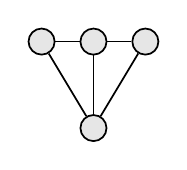
\begin{tikzpicture}[scale=0.5]
[every node/.style={inner sep=0pt}]
\node (4) [circle, minimum size=6pt, fill=cc, line width=0.625pt, draw=black] at (187.5pt, -125.0pt)  {};
\node (3) [circle, minimum size=6pt, fill=cc, line width=0.625pt, draw=black] at (150.0pt, -125.0pt)  {};
\node (2) [circle, minimum size=6pt, fill=cc, line width=0.625pt, draw=black] at (112.5pt, -125.0pt)  {};
\node (1) [circle, minimum size=6pt, fill=cc, line width=0.625pt, draw=black] at (150.0pt, -187.5pt)  {};
\draw [line width=0.625, color=black] (1) to  (3);
\draw [line width=0.625, color=black] (2) to  (3);
\draw [line width=0.625, color=black] (2) to  (1);
\draw [line width=0.625, color=black] (1) to  (4);
\draw [line width=0.625, color=black] (4) to  (3);
\end{tikzpicture}
\end{center}
\end{frame}

\begin{frame}{Deciding whether Graphs are Isomorphic}
	Deciding whether two large graphs are isomorphic is difficult and is an area of active research in Computer Science called The Graph Isomorphism Problem. For smaller graphs it can be done by inspection but there are some tricks which help:

	\begin{alertblock}{Determining isomorphisms}
		\begin{itemize}
			\item Two isomorphic graphs must have the same set of degrees
			\item There must be the same number of loops and multiple edges
		\end{itemize}
		Neither point works in reverse!

	\end{alertblock}
	
	\usetikzlibrary{shapes.geometric}
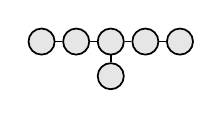
\begin{tikzpicture}[scale=0.5]
[every node/.style={inner sep=0pt}]
\node (1) [circle, minimum size=6pt, fill=cc, line width=0.625pt, draw=black] at (100.0pt, -162.5pt)  {};
\node (2) [circle, minimum size=6pt, fill=cc, line width=0.625pt, draw=black] at (125.0pt, -162.5pt)  {};
\node (3) [circle, minimum size=6pt, fill=cc, line width=0.625pt, draw=black] at (150.0pt, -162.5pt)  {};
\node (4) [circle, minimum size=6pt, fill=cc, line width=0.625pt, draw=black] at (175.0pt, -162.5pt)  {};
\node (5) [circle, minimum size=6pt, fill=cc, line width=0.625pt, draw=black] at (200.0pt, -162.5pt)  {};
\node (6) [circle, minimum size=6pt, fill=cc, line width=0.625pt, draw=black] at (150.0pt, -187.5pt)  {};
\draw [line width=0.625, color=black] (1) to (2);
\draw [line width=0.625, color=black] (2) to (3);
\draw [line width=0.625, color=black] (3) to (4);
\draw [line width=0.625, color=black] (4) to (5);
\draw [line width=0.625, color=black] (3) to (6);
\end{tikzpicture}
\usetikzlibrary{shapes.geometric}
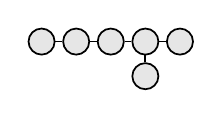
\begin{tikzpicture}[scale=0.5]
[every node/.style={inner sep=0pt}]
\node (1) [circle, minimum size=6pt, fill=cc, line width=0.625pt, draw=black] at (100.0pt, -162.5pt)  {};
\node (2) [circle, minimum size=6pt, fill=cc, line width=0.625pt, draw=black] at (125.0pt, -162.5pt)  {};
\node (3) [circle, minimum size=6pt, fill=cc, line width=0.625pt, draw=black] at (150.0pt, -162.5pt)  {};
\node (4) [circle, minimum size=6pt, fill=cc, line width=0.625pt, draw=black] at (175.0pt, -162.5pt)  {};
\node (5) [circle, minimum size=6pt, fill=cc, line width=0.625pt, draw=black] at (200.0pt, -162.5pt)  {};
\node (6) [circle, minimum size=6pt, fill=cc, line width=0.625pt, draw=black] at (175.0pt, -187.5pt)  {};
\draw [line width=0.625, color=black] (1) to(2);
\draw [line width=0.625, color=black] (2) to(3);
\draw [line width=0.625, color=black] (3) to(4);
\draw [line width=0.625, color=black] (4) to(5);
\draw [line width=0.625, color=black] (4) to(6);
\end{tikzpicture}
These graphs have the set of degrees but the are not isomorphic.

\begin{Problem}
	\begin{minipage}{.6\linewidth}
	Which of the following is isomorphic to this graph?%needed!
	\end{minipage}%
	\begin{minipage}{.4\linewidth}
		\adjustbox{max height=20pt}{
		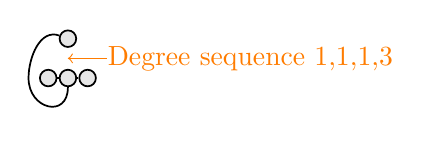
\begin{tikzpicture}
			[scale=0.25,every node/.style={inner sep=0pt}]
			\node (1) [circle, minimum size=6pt, fill=cc, line width=0.625pt, draw=black] at (0, 0)  {};
			\node (2) [circle, minimum size=6pt, fill=cc, line width=0.625pt, draw=black] at (-1, 0)  {};
			\node (3) [circle, minimum size=6pt, fill=cc, line width=0.625pt, draw=black] at (1, 0)  {};
			\node (4) [circle, minimum size=6pt, fill=cc, line width=0.625pt, draw=black] at (0, 2)  {};
			\draw [line width=0.625, color=black] (1) to (2);
			\draw [line width=0.625, color=black] (1) to (3);
			\draw [line width=0.625, color=black] (1) to[in=-90,out=-90,looseness=2] (-2,0) to[out=90,in=160] (4);
			\draw[color=aa,<-] (0,1) -- (2,1) node[right] {Degree sequence 1,1,1,3};
		\end{tikzpicture}}
	\end{minipage}
\end{Problem}

\begin{columns}[T]
	\begin{column}{.5\linewidth}
			\adjustbox{max height=12pt}{
		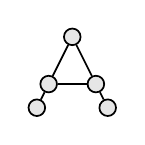
\begin{tikzpicture}
			[scale=0.15,every node/.style={inner sep=0pt}]
			\node (1) [circle, minimum size=6pt, fill=cc, line width=0.625pt, draw=black] at (0, 0)  {};
			\node (2) [circle, minimum size=6pt, fill=cc, line width=0.625pt, draw=black] at (1, 2)  {};
			\node (3) [circle, minimum size=6pt, fill=cc, line width=0.625pt, draw=black] at (3, 6)  {};
			\node (4) [circle, minimum size=6pt, fill=cc, line width=0.625pt, draw=black] at (5, 2)  {};
			\node (5) [circle, minimum size=6pt, fill=cc, line width=0.625pt, draw=black] at (6, 0)  {};
			\draw [line width=0.625, color=black] (1) to (2);
			\draw [line width=0.625, color=black] (2) to (3);
			\draw [line width=0.625, color=black] (2) to (4);
			\draw [line width=0.625, color=black] (3) to (4);
			\draw [line width=0.625, color=black] (4) to (5);
	\end{tikzpicture}}
\sol[2]{Different number of vertices}

			\adjustbox{max height=12pt}{
	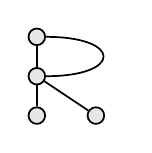
\begin{tikzpicture}
		[scale=0.25,every node/.style={inner sep=0pt}]
		\node (1) [circle, minimum size=6pt, fill=cc, line width=0.625pt, draw=black] at (0, 0)  {};
		\node (2) [circle, minimum size=6pt, fill=cc, line width=0.625pt, draw=black] at (0, 2)  {};
		\node (3) [circle, minimum size=6pt, fill=cc, line width=0.625pt, draw=black] at (0, 4)  {};
		\node (4) [circle, minimum size=6pt, fill=cc, line width=0.625pt, draw=black] at (3, 0)  {};
		\draw [line width=0.625, color=black] (1) to (2);
		\draw [line width=0.625, color=black] (2) to (3);
		\draw [line width=0.625, color=black] (2) to (4);
		\draw [line width=0.625, color=black] (3) to[in=0,out=0,looseness=5] (2);
\end{tikzpicture}}
\sol[3]{Degree sequence 1,1,2,4}
	\end{column}
	\begin{column}{.5\linewidth}
					\adjustbox{max height=12pt}{
			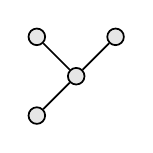
\begin{tikzpicture}
				[scale=0.5,every node/.style={inner sep=0pt}]
				\node (1) [circle, minimum size=6pt, fill=cc, line width=0.625pt, draw=black] at (0, 0)  {};
				\node (2) [circle, minimum size=6pt, fill=cc, line width=0.625pt, draw=black] at (1, 1)  {};
				\node (3) [circle, minimum size=6pt, fill=cc, line width=0.625pt, draw=black] at (0, 2)  {};
				\node (4) [circle, minimum size=6pt, fill=cc, line width=0.625pt, draw=black] at (2, 2)  {};
				\draw [line width=0.625, color=black] (1) to (2);
				\draw [line width=0.625, color=black] (2) to (3);
				\draw [line width=0.625, color=black] (2) to (4);
		\end{tikzpicture}}
		\sol[5]{Yes they are}
		
		\adjustbox{max height=12pt}{
			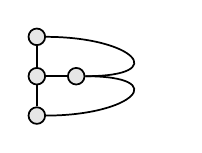
\begin{tikzpicture}
				[scale=0.25,every node/.style={inner sep=0pt}]
				\node (1) [circle, minimum size=6pt, fill=cc, line width=0.625pt, draw=black] at (0, 0)  {};
				\node (2) [circle, minimum size=6pt, fill=cc, line width=0.625pt, draw=black] at (0, 2)  {};
				\node (3) [circle, minimum size=6pt, fill=cc, line width=0.625pt, draw=black] at (0, 4)  {};
				\node (4) [circle, minimum size=6pt, fill=cc, line width=0.625pt, draw=black] at (2, 2)  {};
				\draw [line width=0.625, color=black] (1) to (2);
				\draw [line width=0.625, color=black] (2) to (3);
				\draw [line width=0.625, color=black] (2) to (4);
				\draw [line width=0.625, color=black] (3) to[in=0,out=0,looseness=4] (4);
				\draw [line width=0.625, color=black] (1) to[in=0,out=0,looseness=4] (4);
		\end{tikzpicture}}
		\sol[4]{Degree sequence 3,3,3,3}
	\end{column}
\end{columns}


\end{frame}

\begin{frame}{Giving the Isomorphism}
	\begin{alertblock}{Vertex mapping}
		The isomorphism can be given by explicitly describing which \textbf{vertex maps} to which. 
		
	\end{alertblock}
\begin{Problem}
Are the following graphs isomorphic? Justify your answer.
\usetikzlibrary{shapes.geometric}
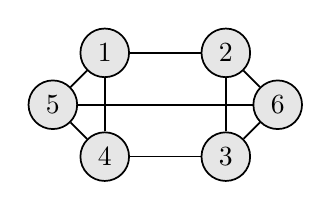
\begin{tikzpicture}[scale=0.5]
[every node/.style={inner sep=0pt}]
\node (1) [circle, minimum size=6pt, fill=cc, line width=0.625pt, draw=black] at (87.5pt, -187.5pt) {\textcolor{black}{1}};
\node (2) [circle, minimum size=6pt, fill=cc, line width=0.625pt, draw=black] at (175.0pt, -187.5pt) {\textcolor{black}{2}};
\node (3) [circle, minimum size=6pt, fill=cc, line width=0.625pt, draw=black] at (175.0pt, -262.5pt) {\textcolor{black}{3}};
\node (4) [circle, minimum size=6pt, fill=cc, line width=0.625pt, draw=black] at (87.5pt, -262.5pt) {\textcolor{black}{4}};
\node (5) [circle, minimum size=6pt, fill=cc, line width=0.625pt, draw=black] at (50.0pt, -225.0pt) {\textcolor{black}{5}};
\node (6) [circle, minimum size=6pt, fill=cc, line width=0.625pt, draw=black] at (212.5pt, -225.0pt) {\textcolor{black}{6}};
\draw [line width=0.625, color=black] (1) to (2);
\draw [line width=0.625, color=black] (2) to (3);
\draw [line width=0.625, color=black] (3) to (4);
\draw [line width=0.625, color=black] (4) to (1);
\draw [line width=0.625, color=black] (1) to (5);
\draw [line width=0.625, color=black] (5) to (6);
\draw [line width=0.625, color=black] (6) to (3);
\draw [line width=0.625, color=black] (2) to (6);
\draw [line width=0.625, color=black] (5) to (4);
\end{tikzpicture}
\usetikzlibrary{shapes.geometric}
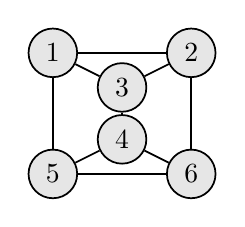
\begin{tikzpicture}[scale=0.5]
[every node/.style={inner sep=0pt}]
\node (1) [circle, minimum size=6pt, fill=cc, line width=0.625pt, draw=black] at (112.5pt, -162.5pt) {\textcolor{black}{1}};
\node (5) [circle, minimum size=6pt, fill=cc, line width=0.625pt, draw=black] at (112.5pt, -250.0pt) {\textcolor{black}{5}};
\node (3) [circle, minimum size=6pt, fill=cc, line width=0.625pt, draw=black] at (162.5pt, -187.5pt) {\textcolor{black}{3}};
\node (4) [circle, minimum size=6pt, fill=cc, line width=0.625pt, draw=black] at (162.5pt, -225.0pt) {\textcolor{black}{4}};
\node (2) [circle, minimum size=6pt, fill=cc, line width=0.625pt, draw=black] at (212.5pt, -162.5pt) {\textcolor{black}{2}};
\node (6) [circle, minimum size=6pt, fill=cc, line width=0.625pt, draw=black] at (212.5pt, -250.0pt) {\textcolor{black}{6}};
\draw [line width=0.625, color=black] (1) to (2);
\draw [line width=0.625, color=black] (1) to (3);
\draw [line width=0.625, color=black] (1) to (5);
\draw [line width=0.625, color=black] (3) to (4);
\draw [line width=0.625, color=black] (3) to (2);
\draw [line width=0.625, color=black] (4) to (6);
\draw [line width=0.625, color=black] (6) to (5);
\draw [line width=0.625, color=black] (4) to (5);
\draw [line width=0.625, color=black] (2) to (6);
\end{tikzpicture}
\end{Problem}	

The degree sequence of both graphs is the same so they have a chance of being isomorphic.

They are isomorphic and the following would be an isomorphism:
\begin{align*}
	1 &\rightarrow A \\
	2 &\rightarrow E \\
	3 &\rightarrow F \\
	4 &\rightarrow B \\
	5 &\rightarrow C \\
	6 &\rightarrow D	
\end{align*}
\end{frame}

\begin{frame}{The Utilities Problem}
	\begin{Problem}
		Suppose there are three houses on a plane and each need to be connected to the gas, water and electricity companies. Without using a third dimension or sending any of the connections through another company or cottage, it there any way of making all nine connections without any of the lines crossing each other?

	\end{Problem}

	The answer is 'No'. Because no matter how you draw the graph above, it will always have some edges that cross. We can say that this is a \textbf{non-planar} graph. 
	
\end{frame}

\begin{frame}{Planar Graphs}
	\begin{alertblock}{Planarity}
		A graph is \textbf{planar} if there is no way to draw it on a 2D plane without the edges crossing.

	\end{alertblock}
	\begin{Problem}
		Show that this is a planar graph.
	
\centering
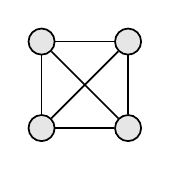
\begin{tikzpicture}[scale=0.5][scale=0.5]
[every node/.style={inner sep=0pt}]
\node (1) [circle, minimum size=6pt, fill=cc, line width=0.625pt, draw=black] at (112.5pt, -125.0pt)  {};
\node (2) [circle, minimum size=6pt, fill=cc, line width=0.625pt, draw=black] at (175.0pt, -125.0pt)  {};
\node (3) [circle, minimum size=6pt, fill=cc, line width=0.625pt, draw=black] at (175.0pt, -187.5pt)  {};
\node (4) [circle, minimum size=6pt, fill=cc, line width=0.625pt, draw=black] at (112.5pt, -187.5pt)  {};
\draw [line width=0.625, color=black] (1) to  (3);
\draw [line width=0.625, color=black] (2) to  (3);
\draw [line width=0.625, color=black] (2) to  (1);
\draw [line width=0.625, color=black] (1) to  (4);
\draw [line width=0.625, color=black] (4) to  (3);
\draw [line width=0.625, color=black] (4) to  (2);
\end{tikzpicture}
	
\end{Problem}

\begin{solution}<2->
We can redraw this graph in such a way that there are no edge crossings.
\centering
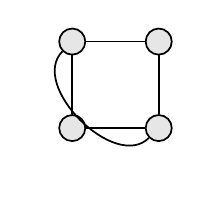
\begin{tikzpicture}[scale=0.5][scale=0.5]
[every node/.style={inner sep=0pt}]
\node (1) [circle, minimum size=6pt, fill=cc, line width=0.625pt, draw=black] at (112.5pt, -125.0pt)  {};
\node (2) [circle, minimum size=6pt, fill=cc, line width=0.625pt, draw=black] at (175.0pt, -125.0pt)  {};
\node (3) [circle, minimum size=6pt, fill=cc, line width=0.625pt, draw=black] at (175.0pt, -187.5pt)  {};
\node (4) [circle, minimum size=6pt, fill=cc, line width=0.625pt, draw=black] at (112.5pt, -187.5pt)  {};
\draw [line width=0.625, color=black] (1) to  [in=225, out=225] (3);
\draw [line width=0.625, color=black] (2) to  (3);
\draw [line width=0.625, color=black] (2) to  (1);
\draw [line width=0.625, color=black] (1) to  (4);
\draw [line width=0.625, color=black] (4) to  (3);
\end{tikzpicture}

Therefore it is planar.
\end{solution}

\end{frame}

\begin{frame}{Kuratowski's Theorem}
\begin{columns}[T]
		\begin{column}{.5\linewidth}
			\centering
			\usetikzlibrary{shapes.geometric}
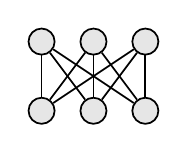
\begin{tikzpicture}[scale=0.5]
[every node/.style={inner sep=0pt}]
\node (1) [circle, minimum size=6pt, fill=cc, line width=0.625pt, draw=black] at (100.0pt, -150.0pt)  {};
\node (2) [circle, minimum size=6pt, fill=cc, line width=0.625pt, draw=black] at (137.5pt, -150.0pt)  {};
\node (3) [circle, minimum size=6pt, fill=cc, line width=0.625pt, draw=black] at (175.0pt, -150.0pt)  {};
\node (4) [circle, minimum size=6pt, fill=cc, line width=0.625pt, draw=black] at (100.0pt, -200.0pt)  {};
\node (5) [circle, minimum size=6pt, fill=cc, line width=0.625pt, draw=black] at (137.5pt, -200.0pt)  {};
\node (6) [circle, minimum size=6pt, fill=cc, line width=0.625pt, draw=black] at (175.0pt, -200.0pt)  {};
\draw [line width=0.625, color=black] (4) to  (1);
\draw [line width=0.625, color=black] (4) to  (2);
\draw [line width=0.625, color=black] (4) to (3);
\draw [line width=0.625, color=black] (5) to (1);
\draw [line width=0.625, color=black] (5) to  (2);
\draw [line width=0.625, color=black] (5) to (3);
\draw [line width=0.625, color=black] (6) to (1);
\draw [line width=0.625, color=black] (6) to (2);
\draw [line width=0.625, color=black] (6) to  (3);
\end{tikzpicture}






\vspace{1cm}


\centering
\usetikzlibrary{shapes.geometric}
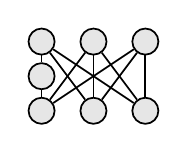
\begin{tikzpicture}[scale=0.5]
[every node/.style={inner sep=0pt}]
\node (1) [circle, minimum size=6pt, fill=cc, line width=0.625pt, draw=black] at (100.0pt, -150.0pt)  {};
\node (2) [circle, minimum size=6pt, fill=cc, line width=0.625pt, draw=black] at (137.5pt, -150.0pt)  {};
\node (3) [circle, minimum size=6pt, fill=cc, line width=0.625pt, draw=black] at (175.0pt, -150.0pt)  {};
\node (4) [circle, minimum size=6pt, fill=cc, line width=0.625pt, draw=black] at (100.0pt, -200.0pt)  {};
\node (5) [circle, minimum size=6pt, fill=cc, line width=0.625pt, draw=black] at (137.5pt, -200.0pt)  {};
\node (6) [circle, minimum size=6pt, fill=cc, line width=0.625pt, draw=black] at (175.0pt, -200.0pt)  {};
\node (7) [circle, minimum size=6pt, fill=cc, line width=0.625pt, draw=black] at (100.0pt, -175.0pt)  {};
\draw [line width=0.625, color=black] (4) to (2);
\draw [line width=0.625, color=black] (4) to (3);
\draw [line width=0.625, color=black] (5) to (1);
\draw [line width=0.625, color=black] (5) to (2);
\draw [line width=0.625, color=black] (5) to (3);
\draw [line width=0.625, color=black] (6) to (1);
\draw [line width=0.625, color=black] (6) to (2);
\draw [line width=0.625, color=black] (6) to  (3);
\draw [line width=0.625, color=black] (4) to  (7);
\draw [line width=0.625, color=black] (7) to (1);
\end{tikzpicture}
		\end{column}


\begin{column}{.5\linewidth}
	\centering
\usetikzlibrary{shapes.geometric}
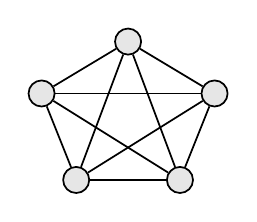
\begin{tikzpicture}[scale=0.5]
[every node/.style={inner sep=0pt}]
\node (1) [circle, minimum size=6pt, fill=cc, line width=0.625pt, draw=black] at (100.0pt, -162.5pt)  {};
\node (4) [circle, minimum size=6pt, fill=cc, line width=0.625pt, draw=black] at (125.0pt, -225.0pt)  {};
\node (5) [circle, minimum size=6pt, fill=cc, line width=0.625pt, draw=black] at (200.0pt, -225.0pt)  {};
\node (2) [circle, minimum size=6pt, fill=cc, line width=0.625pt, draw=black] at (225.0pt, -162.5pt)  {};
\node (3) [circle, minimum size=6pt, fill=cc, line width=0.625pt, draw=black] at (162.5pt, -125.0pt)  {};
\draw [line width=0.625, color=black] (1) to  (3);
\draw [line width=0.625, color=black] (1) to (2);
\draw [line width=0.625, color=black] (1) to (5);
\draw [line width=0.625, color=black] (1) to (4);
\draw [line width=0.625, color=black] (3) to  (2);
\draw [line width=0.625, color=black] (3) to  (5);
\draw [line width=0.625, color=black] (3) to  (4);
\draw [line width=0.625, color=black] (2) to (5);
\draw [line width=0.625, color=black] (2) to (4);
\draw [line width=0.625, color=black] (5) to (4);
\end{tikzpicture}


\centering
\usetikzlibrary{shapes.geometric}
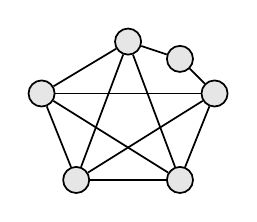
\begin{tikzpicture}[scale=0.5]
[every node/.style={inner sep=0pt}]
\node (1) [circle, minimum size=6pt, fill=cc, line width=0.625pt, draw=black] at (100.0pt, -162.5pt)  {};
\node (4) [circle, minimum size=6pt, fill=cc, line width=0.625pt, draw=black] at (125.0pt, -225.0pt)  {};
\node (5) [circle, minimum size=6pt, fill=cc, line width=0.625pt, draw=black] at (200.0pt, -225.0pt)  {};
\node (2) [circle, minimum size=6pt, fill=cc, line width=0.625pt, draw=black] at (225.0pt, -162.5pt)  {};
\node (3) [circle, minimum size=6pt, fill=cc, line width=0.625pt, draw=black] at (162.5pt, -125.0pt)  {};
\node (6) [circle, minimum size=6pt, fill=cc, line width=0.625pt, draw=black] at (200.0pt, -137.5pt)  {};
\draw [line width=0.625, color=black] (1) to  (3);
\draw [line width=0.625, color=black] (1) to (5);
\draw [line width=0.625, color=black] (1) to (4);
\draw [line width=0.625, color=black] (3) to  (5);
\draw [line width=0.625, color=black] (3) to  (4);
\draw [line width=0.625, color=black] (2) to (5);
\draw [line width=0.625, color=black] (2) to (4);
\draw [line width=0.625, color=black] (5) to (4);
\draw [line width=0.625, color=black] (1) to  (2);
\draw [line width=0.625, color=black] (3) to (6);
\draw [line width=0.625, color=black] (6) to (2);
\end{tikzpicture}
\end{column}

\end{columns}


$K_{3,3}$ cannot be drawn as a planar graph. Clearly a subdivision of it can therefore also not be drawn as a planar graph. This is also why the utilities problem cannot be solved.

$K_5$ cannot be drawn as a planar graph. The same reasoning for a subdivision also holds.

Recall a subdivision of a graph is when a new vertex is added on an edge so that the edge becomes two edges.

\begin{alertblock}{Kuratowski's Theorem}
	A graph is non-planar if and only if it contains a subgraph which can formed by subdividing $K_5$ or  $K_{3,3}$.
\end{alertblock}
\end{frame}

\begin{frame}{Test Your Understanding}
	\begin{columns}[T]
		
\begin{column}{.5\linewidth}
		\begin{Problem}
		Justify whether the following graph is planar. 
		\centering
\usetikzlibrary{shapes.geometric}
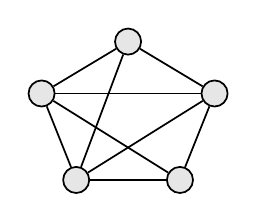
\begin{tikzpicture}[scale=0.5]
[every node/.style={inner sep=0pt}]
\node (1) [circle, minimum size=6pt, fill=cc, line width=0.625pt, draw=black] at (100.0pt, -162.5pt)  {};
\node (4) [circle, minimum size=6pt, fill=cc, line width=0.625pt, draw=black] at (125.0pt, -225.0pt)  {};
\node (5) [circle, minimum size=6pt, fill=cc, line width=0.625pt, draw=black] at (200.0pt, -225.0pt)  {};
\node (2) [circle, minimum size=6pt, fill=cc, line width=0.625pt, draw=black] at (225.0pt, -162.5pt)  {};
\node (3) [circle, minimum size=6pt, fill=cc, line width=0.625pt, draw=black] at (162.5pt, -125.0pt)  {};
\draw [line width=0.625, color=black] (1) to  (3);
\draw [line width=0.625, color=black] (1) to (2);
\draw [line width=0.625, color=black] (1) to (5);
\draw [line width=0.625, color=black] (1) to (4);
\draw [line width=0.625, color=black] (3) to  (2);
\draw [line width=0.625, color=black] (3) to  (4);
\draw [line width=0.625, color=black] (2) to (5);
\draw [line width=0.625, color=black] (2) to (4);
\draw [line width=0.625, color=black] (5) to (4);
\end{tikzpicture}


	\end{Problem}
\begin{solution}<2->
	It is planar as it is $K_5$ with one edge removed, so it cannot have as a subgraph  $K_{3,3}$ or $K_5$ or subdivisions thereof, thus the conclusions follows by Kuratowski's theorem. A suitable rearrangement is below.


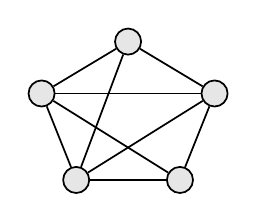
\begin{tikzpicture}[scale=0.5]
[every node/.style={inner sep=0pt}]
\node (1) [circle, minimum size=6pt, fill=cc, line width=0.625pt, draw=black] at (100.0pt, -162.5pt)  {};
\node (4) [circle, minimum size=6pt, fill=cc, line width=0.625pt, draw=black] at (125.0pt, -225.0pt)  {};
\node (5) [circle, minimum size=6pt, fill=cc, line width=0.625pt, draw=black] at (200.0pt, -225.0pt)  {};
\node (2) [circle, minimum size=6pt, fill=cc, line width=0.625pt, draw=black] at (225.0pt, -162.5pt)  {};
\node (3) [circle, minimum size=6pt, fill=cc, line width=0.625pt, draw=black] at (162.5pt, -125.0pt)  {};
\draw [line width=0.625, color=black] (1) to  (3);
\draw [line width=0.625, color=black] (1) to (2);
\draw [line width=0.625, color=black] (1) to (5);
\draw [line width=0.625, color=black] (1) to (4);
\draw [line width=0.625, color=black] (3) to  (2);
\draw [line width=0.625, color=black] (3) to  (4);
\draw [line width=0.625, color=black] (2) to (5);
\draw [line width=0.625, color=black] (2) to (4);
\draw [line width=0.625, color=black] (5) to (4);
\end{tikzpicture}
\end{solution}
\end{column}
\begin{column}{.5\linewidth}
	
\begin{Problem}
	Determine whether or not the following graphs are planar, fully justifying your answer.


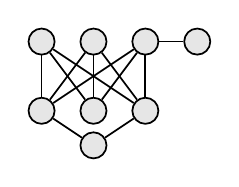
\begin{tikzpicture}[scale=0.5]
[every node/.style={inner sep=0pt}]
\node (1) [circle, minimum size=6pt, fill=cc, line width=0.625pt, draw=black] at (100.0pt, -150.0pt)  {};
\node (2) [circle, minimum size=6pt, fill=cc, line width=0.625pt, draw=black] at (137.5pt, -150.0pt)  {};
\node (3) [circle, minimum size=6pt, fill=cc, line width=0.625pt, draw=black] at (175.0pt, -150.0pt)  {};
\node (4) [circle, minimum size=6pt, fill=cc, line width=0.625pt, draw=black] at (100.0pt, -200.0pt)  {};
\node (5) [circle, minimum size=6pt, fill=cc, line width=0.625pt, draw=black] at (137.5pt, -200.0pt)  {};
\node (6) [circle, minimum size=6pt, fill=cc, line width=0.625pt, draw=black] at (175.0pt, -200.0pt)  {};
\node (7) [circle, minimum size=6pt, fill=cc, line width=0.625pt, draw=black] at (137.5pt, -225.0pt)  {};
\node (8) [circle, minimum size=6pt, fill=cc, line width=0.625pt, draw=black] at (212.5pt, -150.0pt)  {};
\draw [line width=0.625, color=black] (4) to (1);
\draw [line width=0.625, color=black] (4) to (2);
\draw [line width=0.625, color=black] (4) to (3);
\draw [line width=0.625, color=black] (5) to (1);
\draw [line width=0.625, color=black] (5) to  (2);
\draw [line width=0.625, color=black] (5) to  (3);
\draw [line width=0.625, color=black] (6) to (1);
\draw [line width=0.625, color=black] (6) to  (2);
\draw [line width=0.625, color=black] (6) to  (3);
\draw [line width=0.625, color=black] (6) to  (7);
\draw [line width=0.625, color=black] (4) to  (7);
\draw [line width=0.625, color=black] (3) to  (8);
\end{tikzpicture}


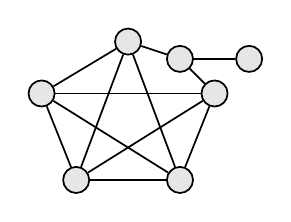
\begin{tikzpicture}[scale=0.5]
[every node/.style={inner sep=0pt}]
\node (1) [circle, minimum size=6pt, fill=cc, line width=0.625pt, draw=black] at (100.0pt, -162.5pt)  {};
\node (4) [circle, minimum size=6pt, fill=cc, line width=0.625pt, draw=black] at (125.0pt, -225.0pt)  {};
\node (5) [circle, minimum size=6pt, fill=cc, line width=0.625pt, draw=black] at (200.0pt, -225.0pt)  {};
\node (2) [circle, minimum size=6pt, fill=cc, line width=0.625pt, draw=black] at (225.0pt, -162.5pt)  {};
\node (3) [circle, minimum size=6pt, fill=cc, line width=0.625pt, draw=black] at (162.5pt, -125.0pt)  {};
\node (6) [circle, minimum size=6pt, fill=cc, line width=0.625pt, draw=black] at (200.0pt, -137.5pt)  {};
\node (7) [circle, minimum size=6pt, fill=cc, line width=0.625pt, draw=black] at (250.0pt, -137.5pt)  {};
\draw [line width=0.625, color=black] (1) to  (3);
\draw [line width=0.625, color=black] (1) to (5);
\draw [line width=0.625, color=black] (1) to  (4);
\draw [line width=0.625, color=black] (3) to  (5);
\draw [line width=0.625, color=black] (3) to  (4);
\draw [line width=0.625, color=black] (2) to  (5);
\draw [line width=0.625, color=black] (2) to  (4);
\draw [line width=0.625, color=black] (5) to  (4);
\draw [line width=0.625, color=black] (1) to  (2);
\draw [line width=0.625, color=black] (3) to (6);
\draw [line width=0.625, color=black] (6) to (2);
\draw [line width=0.625, color=black] (6) to (7);
\end{tikzpicture}
	
\end{Problem}
\begin{solution}<3->
The first one contain $K_{3,3}$ as a subgraph. Hence by Kuratowski's it is non-planar. The second contains a subdivision of $K_5$ as a subgraph hence again by Kuratowski's it is non-planar.
\end{solution}
\end{column}
	\end{columns}

\end{frame}

%In Original there is a past paper question here but since it would take ages to draw 4 graphs i'll let someone else get practice with tikz here.

\begin{frame}[shrink=15]{Faces}
	\begin{alertblock}{Faces}
		\begin{itemize}
			\item A \textbf{face} of a planar graph is an area enclosed by edges
			\item We include the 'outside area' as a face
		\end{itemize}
	\end{alertblock}
\centering
	\usetikzlibrary{shapes.geometric}
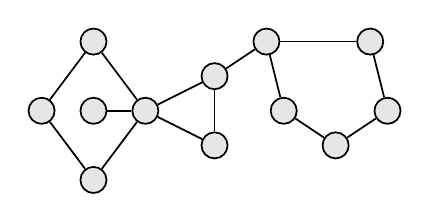
\begin{tikzpicture}[scale=0.5]
[every node/.style={inner sep=0pt}]
\node (1) [circle, minimum size=6pt, fill=cc, line width=0.625pt, draw=black] at (75.0pt, -212.5pt)  {};
\node (2) [circle, minimum size=6pt, fill=cc, line width=0.625pt, draw=black] at (112.5pt, -212.5pt)  {};
\node (3) [circle, minimum size=6pt, fill=cc, line width=0.625pt, draw=black] at (150.0pt, -212.5pt)  {};
\node (4) [circle, minimum size=6pt, fill=cc, line width=0.625pt, draw=black] at (112.5pt, -162.5pt)  {};
\node (5) [circle, minimum size=6pt, fill=cc, line width=0.625pt, draw=black] at (112.5pt, -262.5pt)  {};
\node (6) [circle, minimum size=6pt, fill=cc, line width=0.625pt, draw=black] at (200.0pt, -187.5pt)  {};
\node (7) [circle, minimum size=6pt, fill=cc, line width=0.625pt, draw=black] at (200.0pt, -237.5pt)  {};
\node (8) [circle, minimum size=6pt, fill=cc, line width=0.625pt, draw=black] at (237.5pt, -162.5pt)  {};
\node (9) [circle, minimum size=6pt, fill=cc, line width=0.625pt, draw=black] at (250.0pt, -212.5pt)  {};
\node (10) [circle, minimum size=6pt, fill=cc, line width=0.625pt, draw=black] at (287.5pt, -237.5pt)  {};
\node (11) [circle, minimum size=6pt, fill=cc, line width=0.625pt, draw=black] at (325.0pt, -212.5pt)  {};
\node (12) [circle, minimum size=6pt, fill=cc, line width=0.625pt, draw=black] at (312.5pt, -162.5pt)  {};
\draw [line width=0.625, color=black] (1) to  (4);
\draw [line width=0.625, color=black] (4) to (3);
\draw [line width=0.625, color=black] (1) to (5);
\draw [line width=0.625, color=black] (5) to  (3);
\draw [line width=0.625, color=black] (2) to  (3);
\draw [line width=0.625, color=black] (3) to  (6);
\draw [line width=0.625, color=black] (3) to  (7);
\draw [line width=0.625, color=black] (7) to  (6);
\draw [line width=0.625, color=black] (6) to  (8);
\draw [line width=0.625, color=black] (8) to  (12);
\draw [line width=0.625, color=black] (12) to (11);
\draw [line width=0.625, color=black] (11) to (10);
\draw [line width=0.625, color=black] (10) to (9);
\draw [line width=0.625, color=black] (9) to  (8);
\end{tikzpicture}

A graph with four faces.

\begin{Problem}
	Explain why a tree only has one face.
	
\end{Problem}
\begin{solution}<2->
	
A tree has no cycles. The edges surrounding a face make a cycle. Therefore the only face of a tree is the area around the outside of the graph.

\end{solution}
\begin{Problem}
	Bob claims that two graphs with the same number of vertices, edges and faces must be isomorphic. Find a counter example to Bob's statement. 
\end{Problem}

\begin{solution}<3->
	These graphs both have 4 vertices, 3 edges and 1 face but are not isomorphic. 

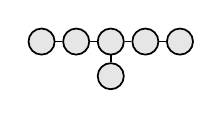
\begin{tikzpicture}[scale=0.5]
[every node/.style={inner sep=0pt}]
\node (1) [circle, minimum size=6pt, fill=cc, line width=0.625pt, draw=black] at (100.0pt, -162.5pt)  {};
\node (2) [circle, minimum size=6pt, fill=cc, line width=0.625pt, draw=black] at (125.0pt, -162.5pt)  {};
\node (3) [circle, minimum size=6pt, fill=cc, line width=0.625pt, draw=black] at (150.0pt, -162.5pt)  {};
\node (4) [circle, minimum size=6pt, fill=cc, line width=0.625pt, draw=black] at (175.0pt, -162.5pt)  {};
\node (5) [circle, minimum size=6pt, fill=cc, line width=0.625pt, draw=black] at (200.0pt, -162.5pt)  {};
\node (6) [circle, minimum size=6pt, fill=cc, line width=0.625pt, draw=black] at (150.0pt, -187.5pt)  {};
\draw [line width=0.625, color=black] (1) to  (2);
\draw [line width=0.625, color=black] (2) to  (3);
\draw [line width=0.625, color=black] (3) to  (4);
\draw [line width=0.625, color=black] (4) to  (5);
\draw [line width=0.625, color=black] (3) to  (6);
\end{tikzpicture}
\usetikzlibrary{shapes.geometric}
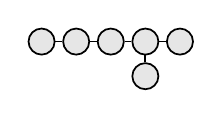
\begin{tikzpicture}[scale=0.5]
[every node/.style={inner sep=0pt}]
\node (1) [circle, minimum size=6pt, fill=cc, line width=0.625pt, draw=black] at (100.0pt, -162.5pt)  {};
\node (2) [circle, minimum size=6pt, fill=cc, line width=0.625pt, draw=black] at (125.0pt, -162.5pt)  {};
\node (3) [circle, minimum size=6pt, fill=cc, line width=0.625pt, draw=black] at (150.0pt, -162.5pt)  {};
\node (4) [circle, minimum size=6pt, fill=cc, line width=0.625pt, draw=black] at (175.0pt, -162.5pt)  {};
\node (5) [circle, minimum size=6pt, fill=cc, line width=0.625pt, draw=black] at (200.0pt, -162.5pt)  {};
\node (6) [circle, minimum size=6pt, fill=cc, line width=0.625pt, draw=black] at (175.0pt, -187.5pt)  {};
\draw [line width=0.625, color=black] (1) to   (2);
\draw [line width=0.625, color=black] (2) to   (3);
\draw [line width=0.625, color=black] (3) to   (4);
\draw [line width=0.625, color=black] (4) to   (5);
\draw [line width=0.625, color=black] (4) to   (6);
\end{tikzpicture}

\end{solution}
\end{frame}

\begin{frame}{Euler's Formula}
	\begin{alertblock}{Euler's Formula}
	For a \emph{connected} planar graph, $v-e+f=2$.
		\begin{itemize}
		\item $v$ is the number of vertices
		\item  $e$ is the number of edges 
		\item $f$ is the number of faces
		\end{itemize}
	\end{alertblock}
\noindent
\begin{minipage}{.5\linewidth}
\usetikzlibrary{shapes.geometric}
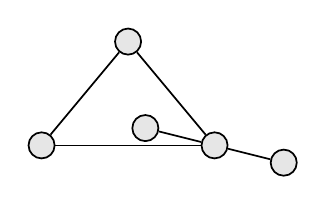
\begin{tikzpicture}[scale=0.5]
[every node/.style={inner sep=0pt}]
\node (1) [circle, minimum size=6pt, fill=cc, line width=0.625pt, draw=black] at (87.5pt, -237.5pt)  {};
\node (2) [circle, minimum size=6pt, fill=cc, line width=0.625pt, draw=black] at (150.0pt, -162.5pt)  {};
\node (3) [circle, minimum size=6pt, fill=cc, line width=0.625pt, draw=black] at (212.5pt, -237.5pt)  {};
\node (4) [circle, minimum size=6pt, fill=cc, line width=0.625pt, draw=black] at (162.5pt, -225.0pt)  {};
\node (5) [circle, minimum size=6pt, fill=cc, line width=0.625pt, draw=black] at (262.5pt, -250.0pt)  {};
\draw [line width=0.625, color=black] (2) to   (1);
\draw [line width=0.625, color=black] (1) to  (3);
\draw [line width=0.625, color=black] (2) to   (3);
\draw [line width=0.625, color=black] (3) to  (4);
\draw [line width=0.625, color=black] (3) to  (5);
\end{tikzpicture}

$v=5,e=5,f=2$
\end{minipage}%
\begin{minipage}{.5\linewidth}
\usetikzlibrary{shapes.geometric}
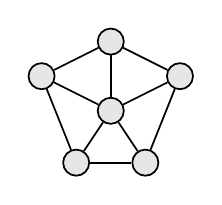
\begin{tikzpicture}[scale=0.5]
[every node/.style={inner sep=0pt}]
\node (1) [circle, minimum size=6pt, fill=cc, line width=0.625pt, draw=black] at (87.5pt, -175.0pt)  {};
\node (2) [circle, minimum size=6pt, fill=cc, line width=0.625pt, draw=black] at (137.5pt, -150.0pt)  {};
\node (3) [circle, minimum size=6pt, fill=cc, line width=0.625pt, draw=black] at (187.5pt, -175.0pt)  {};
\node (4) [circle, minimum size=6pt, fill=cc, line width=0.625pt, draw=black] at (112.5pt, -237.5pt)  {};
\node (5) [circle, minimum size=6pt, fill=cc, line width=0.625pt, draw=black] at (162.5pt, -237.5pt)  {};
\node (6) [circle, minimum size=6pt, fill=cc, line width=0.625pt, draw=black] at (137.5pt, -200.0pt)  {};
\draw [line width=0.625, color=black] (1) to   (2);
\draw [line width=0.625, color=black] (2) to   (3);
\draw [line width=0.625, color=black] (3) to   (5);
\draw [line width=0.625, color=black] (5) to   (4);
\draw [line width=0.625, color=black] (4) to   (1);
\draw [line width=0.625, color=black] (1) to   (6);
\draw [line width=0.625, color=black] (6) to   (2);
\draw [line width=0.625, color=black] (6) to   (3);
\draw [line width=0.625, color=black] (6) to  (5);
\draw [line width=0.625, color=black] (6) to   (4);
\end{tikzpicture}

$v=6,e=10,f=6$
\end{minipage}
\centering
\usetikzlibrary{shapes.geometric}
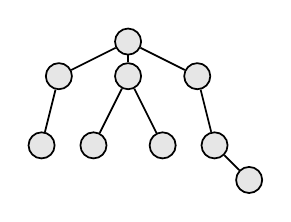
\begin{tikzpicture}[scale=0.5]
[every node/.style={inner sep=0pt}]
\node (1) [circle, minimum size=6pt, fill=cc, line width=0.625pt, draw=black] at (162.5pt, -150.0pt)  {};
\node (2) [circle, minimum size=6pt, fill=cc, line width=0.625pt, draw=black] at (112.5pt, -175.0pt)  {};
\node (3) [circle, minimum size=6pt, fill=cc, line width=0.625pt, draw=black] at (162.5pt, -175.0pt)  {};
\node (4) [circle, minimum size=6pt, fill=cc, line width=0.625pt, draw=black] at (212.5pt, -175.0pt)  {};
\node (5) [circle, minimum size=6pt, fill=cc, line width=0.625pt, draw=black] at (100.0pt, -225.0pt)  {};
\node (6) [circle, minimum size=6pt, fill=cc, line width=0.625pt, draw=black] at (137.5pt, -225.0pt)  {};
\node (7) [circle, minimum size=6pt, fill=cc, line width=0.625pt, draw=black] at (187.5pt, -225.0pt)  {};
\node (8) [circle, minimum size=6pt, fill=cc, line width=0.625pt, draw=black] at (225.0pt, -225.0pt)  {};
\node (9) [circle, minimum size=6pt, fill=cc, line width=0.625pt, draw=black] at (250.0pt, -250.0pt)  {};
\draw [line width=0.625, color=black] (1) to  (2);
\draw [line width=0.625, color=black] (2) to  (5);
\draw [line width=0.625, color=black] (1) to (3);
\draw [line width=0.625, color=black] (3) to (6);
\draw [line width=0.625, color=black] (3) to  (7);
\draw [line width=0.625, color=black] (1) to  (4);
\draw [line width=0.625, color=black] (4) to  (8);
\draw [line width=0.625, color=black] (8) to   (9);
\end{tikzpicture}

\[v=9,e=8,f=1\]

\end{frame}

\begin{frame}{Proof of Euler's Formula}
	We do induction on the number of edges.

	If $e=0$ then because the graph is connected,  $v=1$ and  $f=1$ so
	 \[
	v-e+f=1-0+1=2
	.\] 
	Assume true for $e=k$
	
	If we have a graph with  $e=k+1$ edges, $v$ vertices and  $f$ faces then remove an edge which keeps the graph connected.

	If that edge was part of a cycle, the new graph has  $v$ vertices,  $e-1=k$ edges and $f-1$ faces.
	
	By the induction hypothesis we have that  $v-(e-1)+(f-1)=2$ since $v-e+f=2$.

	If the edge is 'on an end', in order to keep the graph connected we also have to remove the vertex on the end.

	Hence the new graph has  $v-1$ vertices,  $e-1=k$ edges and still  $f$ faces.

	By the induction hypothesis we have that  $(v-1) + (e-1)+f =2$ since $v-e+f=2$.


\end{frame}

\begin{frame}{Test Your Understanding}
	\begin{Problem}
		Determine the number of edges in a connected planar graph with 42 vertices and 40 faces.
	\end{Problem}
\begin{solution}<2->
	
	Euler's formula gives $v-e+f=2$. Hence  $(42)-e+(40)=2$ thus  $e=80$. 
\end{solution}
	\begin{Problem}
		A connected planar graph has $3x+1$ vertices,  $x^2$ edges and $7x+1$ faces. What is  $x$?
	\end{Problem}
\begin{solution}<3->
	
	Using Euler's formula gives, $(3x+1)-(x^2)+(7x+1)=2$. This rearranges to  $x(x-10)=0$. Hence  $x=1 \text{ or } 10$.
\end{solution}
	\begin{Problem}
		How many faces are there in a connected planar graph with 24 vertices, each having degree 3.
		
	\end{Problem}
\begin{solution}<4->
	
	If a vertex has degree 3 it means that 3 edges leave/enter that vertex. So since this will count each edge twice there will be $12 \times 3=36$ edges. Then using Euler's Formula gives,  $(24)-(36)+f=2$. This gives  $f=14$.
\end{solution}

\end{frame}



\begin{frame}{Polyhedra}

	Euler's Formula also means that $v-e+f=2$ for convex polyhedra as they can be 'projected' into a graph.

	%Images needed, Just google Tikz polyhedra

	We can use Euler's formula to prove that there are only five Platonic solids (solids with a regular polygon on each face).
	
\end{frame}

\end{document}
